
%% bare_jrnl.tex
%% V1.4b
%% 2015/08/26
%% by Michael Shell
%% see http://www.michaelshell.org/
%% for current contact information.B8-85-84-AF-15-1B
%%
%% This is a skeleton file demonstrating the use of IEEEtran.cls
%% (requires IEEEtran.cls version 1.8b or later) with an IEEE
%% journal paper.
%%
%% Support sites: %% http://www.michaelshell.org/tex/ieeetran/
%% http://www.ctan.org/pkg/ieeetran
%% and
%% http://www.ieee.org/

%%*************************************************************************
%% Legal Notice:
%% This code is offered as-is without any warranty either expressed or
%% implied; without even the implied warranty of MERCHANTABILITY or
%% FITNESS FOR A PARTICULAR PURPOSE!
%% User assumes all risk.
%% In no event shall the IEEE or any contributor to this code be liable for
%% any damages or losses, including, but not limited to, incidental,
%% consequential, or any other damages, resulting from the use or misuse
%% of any information contained here.
%%
%% All comments are the opinions of their respective authors and are not
%% necessarily endorsed by the IEEE.
%%
%% This work is distributed under the LaTeX Project Public License (LPPL)
%% ( http://www.latex-project.org/ ) version 1.3, and may be freely used,
%% distributed and modified. A copy of the LPPL, version 1.3, is included
%% in the base LaTeX documentation of all distributions of LaTeX released
%% 2003/12/01 or later.
%% Retain all contribution notices and credits.
%% ** Modified files should be clearly indicated as such, including  **
%% ** renaming them and changing author support contact information. **
%%*************************************************************************


% *** Authors should verify (and, if needed, correct) their LaTeX system  ***
% *** with the testflow diagnostic prior to trusting their LaTeX platform ***
% *** with production work. The IEEE's font choices and paper sizes can   ***
% *** trigger bugs that do not appear when using other class files.       ***                          ***
% The testflow support page is at:
% http://www.michaelshell.org/tex/testflow/



\documentclass[journal]{IEEEtran}
%
% If IEEEtran.cls has not been installed into the LaTeX system files,
% manually specify the path to it like:
% \documentclass[journal]{../sty/IEEEtran}





% Some very useful LaTeX packages include:
% (uncomment the ones you want to load)


% *** MISC UTILITY PACKAGES ***
%
%\usepackage{ifpdf}
% Heiko Oberdiek's ifpdf.sty is very useful if you need conditional
% compilation based on whether the output is pdf or dvi.
% usage:
% \ifpdf
%   % pdf code
% \else
%   % dvi code
% \fi
% The latest version of ifpdf.sty can be obtained from:
% http://www.ctan.org/pkg/ifpdf
% Also, note that IEEEtran.cls V1.7 and later provides a builtin
% \ifCLASSINFOpdf conditional that works the same way.
% When switching from latex to pdflatex and vice-versa, the compiler may
% have to be run twice to clear warning/error messages.






% *** CITATION PACKAGES ***
%
%\usepackage{cite}
% cite.sty was written by Donald Arseneau
% V1.6 and later of IEEEtran pre-defines the format of the cite.sty package
% \cite{} output to follow that of the IEEE. Loading the cite package will
% result in citation numbers being automatically sorted and properly
% "compressed/ranged". e.g., [1], [9], [2], [7], [5], [6] without using
% cite.sty will become [1], [2], [5]--[7], [9] using cite.sty. cite.sty's
% \cite will automatically add leading space, if needed. Use cite.sty's
% noadjust option (cite.sty V3.8 and later) if you want to turn this off
% such as if a citation ever needs to be enclosed in parenthesis.
% cite.sty is already installed on most LaTeX systems. Be sure and use
% version 5.0 (2009-03-20) and later if using hyperref.sty.
% The latest version can be obtained at:
% http://www.ctan.org/pkg/cite
% The documentation is contained in the cite.sty file itself.






% *** GRAPHICS RELATED PACKAGES ***
%
\ifCLASSINFOpdf
  % \usepackage[pdftex]{graphicx}
  % declare the path(s) where your graphic files are
  % \graphicspath{{../pdf/}{../jpeg/}}
  % and their extensions so you won't have to specify these with
  % every instance of \includegraphics
  % \DeclareGraphicsExtensions{.pdf,.jpeg,.png}
\else
  % or other class option (dvipsone, dvipdf, if not using dvips). graphicx
  % will default to the driver specified in the system graphics.cfg if no
  % driver is specified.
  % \usepackage[dvips]{graphicx}
  % declare the path(s) where your graphic files are
  % \graphicspath{{../eps/}}
  % and their extensions so you won't have to specify these with
  % every instance of \includegraphics
  % \DeclareGraphicsExtensions{.eps}
\fi
% graphicx was written by David Carlisle and Sebastian Rahtz. It is
% required if you want graphics, photos, etc. graphicx.sty is already
% installed on most LaTeX systems. The latest version and documentation
% can be obtained at:
% http://www.ctan.org/pkg/graphicx
% Another good source of documentation is "Using Imported Graphics in
% LaTeX2e" by Keith Reckdahl which can be found at:
% http://www.ctan.org/pkg/epslatex
%
% latex, and pdflatex in dvi mode, support graphics in encapsulated
% postscript (.eps) format. pdflatex in pdf mode supports graphics
% in .pdf, .jpeg, .png and .mps (metapost) formats. Users should ensure
% that all non-photo figures use a vector format (.eps, .pdf, .mps) and
% not a bitmapped formats (.jpeg, .png). The IEEE frowns on bitmapped formats
% which can result in "jaggedy"/blurry rendering of lines and letters as
% well as large increases in file sizes.
%
% You can find documentation about the pdfTeX application at:
% http://www.tug.org/applications/pdftex


\usepackage{color}
\usepackage{amsmath}
\usepackage{amssymb}
\usepackage{tabularx}

\usepackage{epsfig}
%\usepackage[colorlinks=false, urlcolor=black, pdfborder={0 0 0}]{hyperref}
%\let\url\nolinkurl
%\usepackage[options]{nohyperref}  % This makes hyperref commands do nothing without errors
\usepackage{url}  % This makes \url work

%\usepackage[dvips]{epsfig}
\usepackage{etoolbox}
\apptocmd{\sloppy}{\hbadness 10000\relax}{}{}

\usepackage{longtable}
\usepackage{graphicx}
\usepackage[T1]{fontenc}
\usepackage{paralist}
\usepackage{enumitem}
%%%%%%%%%%%%for
\usepackage{adjustbox}
\usepackage{array}
\usepackage{booktabs}
\newcolumntype{C}{>{\centering\arraybackslash}X} % centered version of "X" type
\setlength{\extrarowheight}{1pt}
%\usepackage{lipsum}
\usepackage{multirow}

\newcolumntype{R}[2]{%
    >{\adjustbox{angle=#1,lap=\width-(#2)}\bgroup}%
    l%
    <{\egroup}%
}
\newcommand*\rot{\multicolumn{1}{R{90}{1em}}}% no optional argument here, please!

\usepackage{epstopdf}


\def\BibTeX{{\rm B\kern-.05em{\sc i\kern-.025em b}\kern-.08em
    T\kern-.1667em\lower.7ex\hbox{E}\kern-.125emX}}

\usepackage{pdflscape}
%\usepackage{subfigure}
\usepackage{tabularx}
\usepackage{xtab}
%\usepackage{supertabular}

\usepackage{booktabs, threeparttable}
\usepackage{array}
\newcolumntype{L}[1]{>{\raggedright\arraybackslash}p{#1}}

% *** MATH PACKAGES ***
\usepackage{algorithm}
\usepackage[noend]{algpseudocode}

\makeatletter
\def\BState{\State\hskip-\ALG@thistlm}
\makeatother

\algnewcommand\algorithmicswitch{\textbf{switch}}
\algnewcommand\algorithmiccase{\textbf{case}}
\algnewcommand\algorithmicassert{\texttt{assert}}
\algnewcommand\Assert[1]{\State \algorithmicassert(#1)}%
% New "environments"
\algdef{SE}[SWITCH]{Switch}{EndSwitch}[1]{\algorithmicswitch\ #1\ \algorithmicdo}{\algorithmicend\ \algorithmicswitch}%
\algdef{SE}[CASE]{Case}{EndCase}[1]{\algorithmiccase\ #1}{\algorithmicend\ \algorithmiccase}%
\algtext*{EndSwitch}%
\algtext*{EndCase}%





% *** SPECIALIZED LIST PACKAGES ***
%
%\usepackage{algorithmic}
% algorithmic.sty was written by Peter Williams and Rogerio Brito.
% This package provides an algorithmic environment fo describing algorithms.
% You can use the algorithmic environment in-text or within a figure
% environment to provide for a floating algorithm. Do NOT use the algorithm
% floating environment provided by algorithm.sty (by the same authors) or
% algorithm2e.sty (by Christophe Fiorio) as the IEEE does not use dedicated
% algorithm float types and packages that provide these will not provide
% correct IEEE style captions. The latest version and documentation of
% algorithmic.sty can be obtained at:
% http://www.ctan.org/pkg/algorithms
% Also of interest may be the (relatively newer and more customizable)
% algorithmicx.sty package by Szasz Janos:
% http://www.ctan.org/pkg/algorithmicx




% *** ALIGNMENT PACKAGES ***
%
%\usepackage{array}
% Frank Mittelbach's and David Carlisle's array.sty patches and improves
% the standard LaTeX2e array and tabular environments to provide better
% appearance and additional user controls. As the default LaTeX2e table
% generation code is lacking to the point of almost being broken with
% respect to the quality of the end results, all users are strongly
% advised to use an enhanced (at the very least that provided by array.sty)
% set of table tools. array.sty is already installed on most systems. The
% latest version and documentation can be obtained at:
% http://www.ctan.org/pkg/array


% IEEEtran contains the IEEEeqnarray family of commands that can be used to
% generate multiline equations as well as matrices, tables, etc., of high
% quality.




% *** SUBFIGURE PACKAGES ***
%\ifCLASSOPTIONcompsoc
%  \usepackage[caption=false,font=normalsize,labelfont=sf,textfont=sf]{subfig}
%\else
%  \usepackage[caption=false,font=footnotesize]{subfig}
%\fi
% subfig.sty, written by Steven Douglas Cochran, is the modern replacement
% for subfigure.sty, the latter of which is no longer maintained and is
% incompatible with some LaTeX packages including fixltx2e. However,
% subfig.sty requires and automatically loads Axel Sommerfeldt's caption.sty
% which will override IEEEtran.cls' handling of captions and this will result
% in non-IEEE style figure/table captions. To prevent this problem, be sure
% and invoke subfig.sty's "caption=false" package option (available since
% subfig.sty version 1.3, 2005/06/28) as this is will preserve IEEEtran.cls
% handling of captions.
% Note that the Computer Society format requires a larger sans serif font
% than the serif footnote size font used in traditional IEEE formatting
% and thus the need to invoke different subfig.sty package options depending
% on whether compsoc mode has been enabled.
%
% The latest version and documentation of subfig.sty can be obtained at:
% http://www.ctan.org/pkg/subfig




% *** FLOAT PACKAGES ***
%
%\usepackage{fixltx2e}
% fixltx2e, the successor to the earlier fix2col.sty, was written by
% Frank Mittelbach and David Carlisle. This package corrects a few problems
% in the LaTeX2e kernel, the most notable of which is that in current
% LaTeX2e releases, the ordering of single and double column floats is not
% guaranteed to be preserved. Thus, an unpatched LaTeX2e can allow a
% single column figure to be placed prior to an earlier double column
% figure.
% Be aware that LaTeX2e kernels dated 2015 and later have fixltx2e.sty's
% corrections already built into the system in which case a warning will
% be issued if an attempt is made to load fixltx2e.sty as it is no longer
% needed.
% The latest version and documentation can be found at:
% http://www.ctan.org/pkg/fixltx2e


%\usepackage{stfloats}
% stfloats.sty was written by Sigitas Tolusis. This package gives LaTeX2e
% the ability to do double column floats at the bottom of the page as well
% as the top. (e.g., "\begin{figure*}[!b]" is not normally possible in
% LaTeX2e). It also provides a command:
%\fnbelowfloat
% to enable the placement of footnotes below bottom floats (the standard
% LaTeX2e kernel puts them above bottom floats). This is an invasive package
% which rewrites many portions of the LaTeX2e float routines. It may not work
% with other packages that modify the LaTeX2e float routines. The latest
% version and documentation can be obtained at:
% http://www.ctan.org/pkg/stfloats
% Do not use the stfloats baselinefloat ability as the IEEE does not allow
% \baselineskip to stretch. Authors submitting work to the IEEE should note
% that the IEEE rarely uses double column equations and that authors should try
% to avoid such use. Do not be tempted to use the cuted.sty or midfloat.sty
% packages (also by Sigitas Tolusis) as the IEEE does not format its papers in
% such ways.
% Do not attempt to use stfloats with fixltx2e as they are incompatible.
% Instead, use Morten Hogholm'a dblfloatfix which combines the features
% of both fixltx2e and stfloats:
%
% \usepackage{dblfloatfix}
% The latest version can be found at:
% http://www.ctan.org/pkg/dblfloatfix




%\ifCLASSOPTIONcaptionsoff
%  \usepackage[nomarkers]{endfloat}
% \let\MYoriglatexcaption\caption
% \renewcommand{\caption}[2][\relax]{\MYoriglatexcaption[#2]{#2}}
%\fi
% endfloat.sty was written by James Darrell McCauley, Jeff Goldberg and
% Axel Sommerfeldt. This package may be useful when used in conjunction with
% IEEEtran.cls'  captionsoff option. Some IEEE journals/societies require that
% submissions have lists of figures/tables at the end of the paper and that
% figures/tables without any captions are placed on a page by themselves at
% the end of the document. If needed, the draftcls IEEEtran class option or
% \CLASSINPUTbaselinestretch interface can be used to increase the line
% spacing as well. Be sure and use the nomarkers option of endfloat to
% prevent endfloat from "marking" where the figures would have been placed
% in the text. The two hack lines of code above are a slight modification of
% that suggested by in the endfloat docs (section 8.4.1) to ensure that
% the full captions always appear in the list of figures/tables - even if
% the user used the short optional argument of \caption[]{}.
% IEEE papers do not typically make use of \caption[]'s optional argument,
% so this should not be an issue. A similar trick can be used to disable
% captions of packages such as subfig.sty that lack options to turn off
% the subcaptions:
% For subfig.sty:
% \let\MYorigsubfloat\subfloat
% \renewcommand{\subfloat}[2][\relax]{\MYorigsubfloat[]{#2}}
% However, the above trick will not work if both optional arguments of
% the \subfloat command are used. Furthermore, there needs to be a
% description of each subfigure *somewhere* and endfloat does not add
% subfigure captions to its list of figures. Thus, the best approach is to
% avoid the use of subfigure captions (many IEEE journals avoid them anyway)
% and instead reference/explain all the subfigures within the main caption.
% The latest version of endfloat.sty and its documentation can obtained at:
% http://www.ctan.org/pkg/endfloat
%
% The IEEEtran \ifCLASSOPTIONcaptionsoff conditional can also be used
% later in the document, say, to conditionally put the References on a
% page by themselves.




% *** PDF, URL AND HYPERLINK PACKAGES ***
%
%\usepackage{url}
% url.sty was written by Donald Arseneau. It provides better support for
% handling and breaking URLs. url.sty is already installed on most LaTeX
% systems. The latest version and documentation can be obtained at:
% http://www.ctan.org/pkg/url
% Basically, \url{my_url_here}.




% *** Do not adjust lengths that control margins, column widths, etc. ***
% *** Do not use packages that alter fonts (such as pslatex).         ***
% There should be no need to do such things with IEEEtran.cls V1.6 and later.
% (Unless specifically asked to do so by the journal or conference you plan
% to submit to, of course. )


% correct bad hyphenation here
%\hyphenation{op-tical net-works semi-conduc-tor}


\begin{document}
%
% paper title
% Titles are generally capitalized except for words such as a, an, and, as,
% at, but, by, for, in, nor, of, on, or, the, to and up, which are usually
% not capitalized unless they are the first or last word of the title.
% Linebreaks \\ can be used within to get better formatting as desired.
% Do not put math or special symbols in the title.
\title{Fully-Decentralised Multi-agent Reinforcement Learning in Fog-based Internet-of-Things}
%
%
% author names and IEEE memberships
% note positions of commas and nonbreaking spaces ( ~ ) LaTeX will not break
% a structure at a ~ so this keeps an author's name from being broken across
% two lines.
% use \thanks{} to gain access to the first footnote area
% a separate \thanks must be used for each paragraph as LaTeX2e's \thanks
% was not built to handle multiple paragraphs
%

\author{XXX~YYYY,
        and~ XXX~ZZZZ% <-this % stops a space
%\thanks{B. Omoniwa is with National Mathematical Centre, PMB 118, Abuja-Nigeria, email: tunjiomoniwa@gmail.com.}% <-this % stops a space

\thanks{Manuscript received March 14, 2019; revised July X, 2019.}
\thanks{Copyright (c) 2012 IEEE. Personal use of this material is permitted. However, permission to use this material for any other purposes must be obtained from the IEEE by sending a request to pubs-permissions@ieee.org.}
}

% note the % following the last \IEEEmembership and also \thanks -
% these prevent an unwanted space from occurring between the last author name
% and the end of the author line. i.e., if you had this:
%
% \author{....lastname \thanks{...} \thanks{...} }
%                     ^------------^------------^----Do not want these spaces!
%
% a space would be appended to the last name and could cause every name on that
% line to be shifted left slightly. This is one of those "LaTeX things". For
% instance, "\textbf{A} \textbf{B}" will typeset as "A B" not "AB". To get
% "AB" then you have to do: "\textbf{A}\textbf{B}"
% \thanks is no different in this regard, so shield the last } of each \thanks
% that ends a line with a % and do not let a space in before the next \thanks.
% Spaces after \IEEEmembership other than the last one are OK (and needed) as
% you are supposed to have spaces between the names. For what it is worth,
% this is a minor point as most people would not even notice if the said evil
% space somehow managed to creep in.



% The paper headers
\markboth{IEEE Internet of Things Journal,~Vol.~X, No.~X, August~2019}%
{YYYY \MakeLowercase{\textit{et al.}}: Fully-Decentralised Multi-agent Reinforcement Learning in Fog-based Internet-of-Things}
% The only time the second header will appear is for the odd numbered pages
% after the title page when using the twoside option.
%
% *** Note that you probably will NOT want to include the author's ***
% *** name in the headers of peer review papers.                   ***
% You can use \ifCLASSOPTIONpeerreview for conditional compilation here if
% you desire.




% If you want to put a publisher's ID mark on the page you can do it like
% this:
%\IEEEpubid{0000--0000/00\$00.00~\copyright~2015 IEEE}
% Remember, if you use this you must call \IEEEpubidadjcol in the second
% column for its text to clear the IEEEpubid mark.



% use for special paper notices
%\IEEEspecialpapernotice{(Invited Paper)}



% make the title area
\maketitle

% As a general rule, do not put math, special symbols or citations
% in the abstract or keywords.
\begin{abstract}
Reinforcement learning (RL) algorithms 

\end{abstract}

% Note that keywords are not normally used for peerreview papers.
\begin{IEEEkeywords}
Reinforcement learning (RL), Internet-of-Things (IoT), Fog-based IoT, Markov decision process (MDP), machine learning (ML).
\end{IEEEkeywords}






% For peer review papers, you can put extra information on the cover
% page as needed:
% \ifCLASSOPTIONpeerreview
% \begin{center} \bfseries EDICS Category: 3-BBND \end{center}
% \fi
%
% For peerreview papers, this IEEEtran command inserts a page break and
% creates the second title. It will be ignored for other modes.
\IEEEpeerreviewmaketitle

\section{Background}
\IEEEPARstart{T}{he} rapid increase in the use of wireless devices and technologies for Internet-of-Things (IoT) applications, such as Industrial IoT, military surveillance, health monitoring, and smart cities, has brought about an increasing need for frameworks on connectivity prediction, information control, and failure analysis to improve network reliability~\cite{Wetzker2016}. Interestingly, with the proliferation of more IoT devices, which widely make use of the unlicensed industrial, scientific, and medical (ISM) frequency band, it is anticipated that the shared frequency spectrum will become more crowded as more and more devices will contend for the wireless medium, resulting poor network performance and increased application failures.

Fog computing platform extends the cloud by bring processing, computation, decision making and control closer to the edge of the network~\cite{Omoniwa2018}. First, the IoT paradigm can effectively leverage on fog devices to deliver reliable network performance by minimizing communication outages caused by poor communication link between communicating parties, and also handle cross-technology interference (CTI) caused by heterogonously deployed IoT devices. Second, via local control, the fog devices can help in extending the longevity of the IoT network.
 



\section{Problem Definition}
In this section, we provide full description of the system model, as well the RL approach used to address the problem. The Mobile Fog Relay Agent (MFRA) and its environment are discussed below.

\subsection{MFRA environment}
\emph{\textbf{States}}: The states are defined as a tuple, $\langle$Outage communication cost ($\mathcal{P}_{out}$) /Energy status of the fog relay (J) /Energy status of the IoT sensor (J)$\rangle$.

\begin{itemize}
  \item Outage communication cost: Outage observations from the environment is estimated using (\ref{eqn1a}) from \cite{OmoniwaRelay2018}, which gives an estimate of the communication outage when the agent takes an action, such as changing power levels or location, or both.
  \item Energy expended by fog relay: This observation gives the agent insight on how much energy by the fog agent when following policy~$\omega_i \in \omega_{fog}$. If the fog agent continues to take sub-optimal actions, it depletes its energy and dies out.
  \item Energy expended by IoT sensor: This observation gives the agent insight on how much energy the IoT sensor has used up by following a policy~$\omega_i \in \omega_{IoT}$. If the IoT sensor continues to take sub-optimal actions, it depletes its energy and dies out.
\end{itemize}


\begin{equation}\label{eqn1a}
  \mathcal{P}_{out} = 1 - (1 + 2\Psi^2 \ln \Psi) \exp\Big( -\frac{N_0 \tilde{\kappa}}{P_{I} (D_{I} + \delta)^{-\sigma}}\Big),
\end{equation}


where~$\Psi = \sqrt{(N_0 \tilde{\kappa})/(P_{R}(D_{S} + \delta)^{-\sigma})}$, and~$\mathcal{P}_{out}$ is an expression for the outage probability with values between 0 and 1. We assume a predefined threshold~$\tilde{\kappa}$ which determines the outage in communication,~$P_{I}$ is transmit power of the IoT sensor,~$P_{R}$ is transmit power of the fog relay agent,~$D_{I}$ is the distance between IoT sensor and fog relay agent, and~$D_{S}$ is the distance between fog relay agent and destination node. We assume a small change in the position of the fog relay agent,~$\delta = \pm0.25 m$,~$N_0$ to be the channel noise, and~$\sigma$ to be the path-loss exponent.



\subsection{MRFA agent}
We apply a the Q-Learning algorithm, an RL approach which requires no prior knowledge of the environment by the agent. In Q-learning, the agent interacts with the environment over periods of time according to a policy~$\omega$. At every time-step~$k \in N$, the environment produces an observation~$s_{k} \in \mathbb{R}^{D_s}$. By sampling, the agent then picks an action~$a_{k}$ over~$\omega(s_{k})$,~$a_{k} \in \mathbb{R}^{D_a}$, which is applied to the environment. The environment consequently produces a reward~$r(s_{k}, a_{k})$ and may end the episode at state~$s_{N}$ or transits to a new state~$s_{k + 1}$. The agent's goal is to minimize the expected cumulative cost,~$\min_{\omega} \mathbb{E}_{s_0, a_0, s_1, a_1, ..., s_N} \Big[ \sum_{i=0}^{N} \gamma^i \mathcal{C}(s_i) \Big]$, where~$0 \leq \gamma \leq 1$ is the discount factor, and~$\mathcal{C}$ is the overall cost function of our model.

First, the agent takes an initial random action~$a_{k}$ and gets observations from the environment which corresponds to that action, as well as a reward. It then discretizes the continuous observations emanating from the environment into a~$50 \times 10 \times 10$ state space corresponding to the tuple, $\langle$Outage communication cost ($\mathcal{P}_{out}$) /Energy status of the fog relay (J) /Energy status of the IoT sensor (J)$\rangle$. The agent then updates it's Q-values at each time-step~$k$ following (\ref{eqn1b}).

\begin{equation}\label{eqn1b}
\begin{split}
Q(s_k, a_k) &:= Q(s_k, a_k)\\
& + \alpha \Big[ r_{k + 1} + \gamma \max_{a}  Q(s_{k + 1}, a) -  Q(s_k, a_k) \Big],
   \end{split}
\end{equation}
where~$\alpha$ is the learning rate, which determines the impact of new experience on the Q-value,~$r_{k + 1}$ is the reward the agent receives by being in~$s_{k + 1}$ from~$s_{k}$. Based on the policy followed by the agent, it gets observations and rewards from the environment.

\emph{\textbf{Action space}}: The actions are move and transmit by fog relay, and select a power-level and transmit by IoT end-device, which make up eight possible actions.

 \begin{itemize}
  \item Mobility: Move by $\pm \delta$ and transmit, where~$\delta = \pm0.25m$ and mobility range (m) = [-30, 30]
  \item Power-level: Choose power-level and transmit, $P$, where~transmit power ranges (W) = [0.001, 0.01, 0.15, 0.2, 0.25, 0.3]
\end{itemize}

\emph{\textbf{Goal}}: The goal is for the agent to learn to minimize the overall cost~$\mathcal{C}$ in the tuple, $\langle$Outage communication cost ($\mathcal{P}_{out}$) /Energy status of the fog relay (J) /Energy status of the IoT sensor (J)$\rangle$, by keeping all nodes within the link alive while ensuring that the packets received in each transmission does not fall below the pre-defined threshold, which was set at 95\%.

\emph{\textbf{Rewards}}: The reward function used is given in (\ref{eqn1b}) as

 \begin{equation}\label{eqn1b}
    R =
    \begin{cases}
      100, & \text{if}\ goal==Reached \\
      0, & \text{otherwise.}
    \end{cases}
  \end{equation}


\emph{\textbf{Metrics}}: Outage probability, i.e. the ratio of the number of packet lost to those transmitted, which we measure in percentages, and energy status of the fog relay agent and the IoT sensor, i.e. the ratio of depleted energy to the initial capacity in Joules, which we measure as a percentage.


The MFRA's learning process is summarized in Algorithm \ref{fiotRL}. A new learning episode is terminated when the agent attains the pre-defined goal of minimizing the communication outage in the link, or when either the fog relay or the IoT sensor dies out due to taking sub-optimal actions without getting to the goal. When an fog relay moves closer to the communicating parties, the IoT sensor uses a lower power level as compared to when it is far away, hereby saving IoT sensor energy. However, mobility have some cost and if the fog relay continues to move in order to minimize the communication outage, it may die out soon, hereby causing a point-of-failure to the network. As each episode is completed, a reward of 100 points is given to the agent if it reaches its goal and a 0 points otherwise. The reward is updated in the Q-learning table, with environmental information updated as well.

\begin{algorithm}
\caption{MFRA Learning Process}\label{fiotRL}
\begin{algorithmic}[1]
\State \textbf{Initialize:} Power levels (W) = [0.001, 0.01, 0.15, 0.2, 0.25, 0.3],~$\delta = \pm0.25m$ and mobility range (m) = [-30, 30]
\BState \emph{top}:
\State ResetEnvironment()
\State \emph{state} $\leftarrow$ MapLocalObservationToState(\emph{env})
\State \emph{action} $\leftarrow$ QLearning.SelectAction(\emph{state})
%\BState \emph{top}:
\If { \emph{action}  == ``move close and Tx''} %\Return stop,
\State Env.EstimateOutage (\ref{eqn1a})
\State Env.EstimateFogEnergyStatus
\ElsIf {\emph{action}  == ``move away and Tx''}
\State Env.EstimateOutage (\ref{eqn1a})
\State Env.EstimateSensorEnergyStatus
\ElsIf { \emph{action}  == ``choose power level and Tx''}
\State Env.EstimateOutage (\ref{eqn1a})
\State Env.EstimateSensorEnergyStatus
\EndIf
\State \textbf{endif}
\State InvokePolicy(ExponentialDecay)
\State UpdateQLearningProcedure() (\ref{eqn1b})
\State CurrentState $\leftarrow$ NewState
\If { \emph{goal}  == ``Reached''}  \Return Reward = 100,
\ElsIf { \emph{goal}  != ``Reached'' or Agent == Death}  \Return Reward = 0
\EndIf
\State \textbf{endif}
\State EndEpisode \textbf{goto} \emph{top}.
\end{algorithmic}
\end{algorithm}







%
%\begin{figure}[!t]
%\centering
%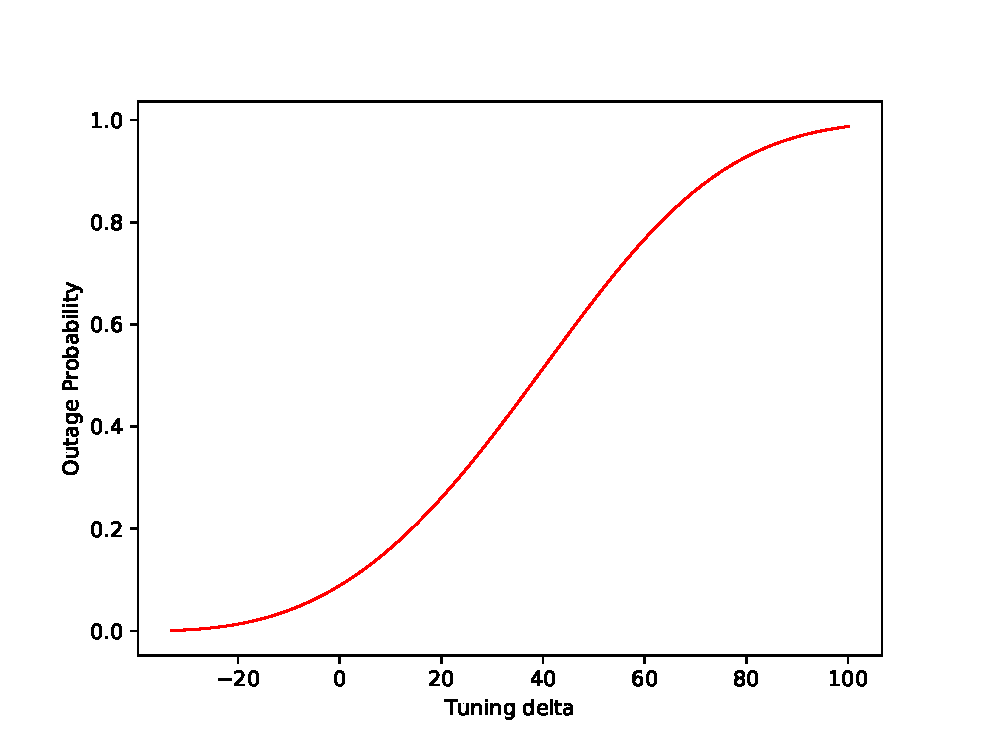
\includegraphics[width=3.8in]{delta_plot.eps}
% %where an .eps filename suffix will be assumed under latex,
%% and a .pdf suffix will be assumed for pdflatex; or what has been declared
%% via \DeclareGraphicsExtensions.
%\caption{Model relationship showing the outage observation w.r.t. change in position of fog agent.}
%\label{delta_plot}
%\end{figure}
%
%
%\begin{figure}[!t]
%\centering
%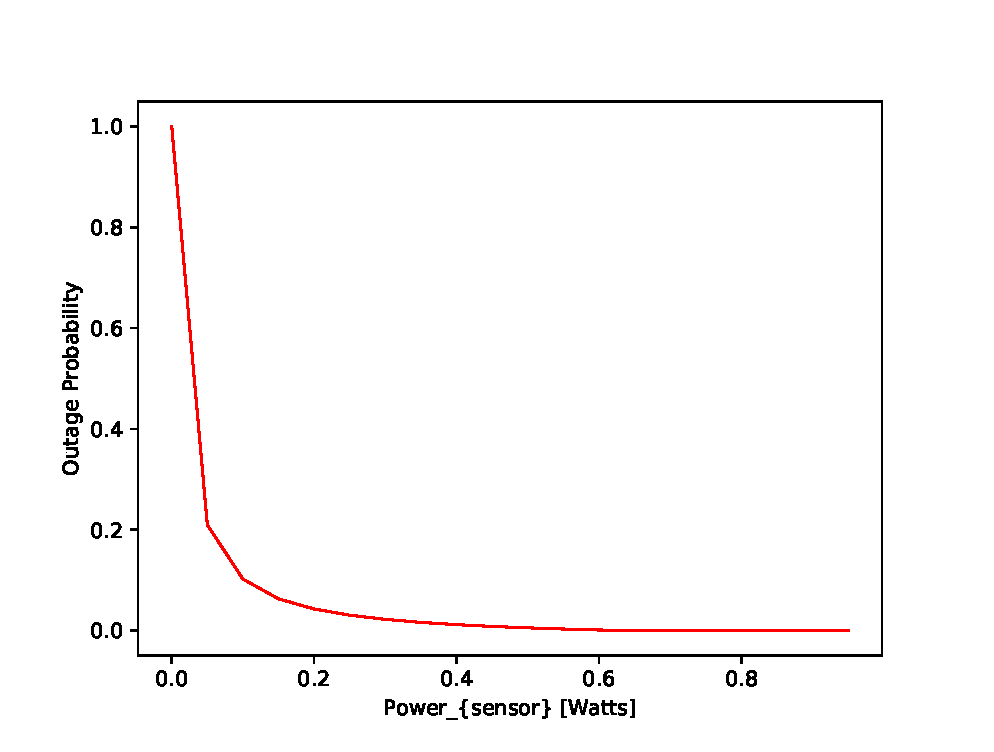
\includegraphics[width=3.8in]{power_plot.eps}
% %where an .eps filename suffix will be assumed under latex,
%% and a .pdf suffix will be assumed for pdflatex; or what has been declared
%% via \DeclareGraphicsExtensions.
%\caption{Model relationship showing the outage observation w.r.t. change in power level of the IoT end-device.}
%\label{power_plot}
%\end{figure}



\section{Experimental Setup}

\subsection{General settings}
We carried out experimentation with 150 fog relays and 1000 IoT sensors randomly deployed.




Table~\ref{table:simparameters} shows a summary of the parameters used in simulating

\begin{table}
\small
\centering
\caption{Simulation Parameters}
\label{table:simparameters}
\begin{tabular}{ll}
  \hline
 \textit{Parameter} & \textit{Values} \\
  \hline \hline

   $D_{I}$ & 40 metres\\
   $P_{I}$ & [0.001, 0.3] Watts \\
   $D_{S}$ & 35 metres\\
   $P_{R}$ & 0.3 Watts\\
   $\delta$ & $\pm0.25$ metres\\
   Mobility bound & [-35,~35] metres\\
   Noise power $N_0$ & $2 \times 10^{-7}$ Watts\\
   Path-loss exponent $\sigma$ & 3\\
   Pre-defined threshold $\kappa$ & 1\\
   Discount factor $\gamma$ & 0.9\\
   Learning rate $\alpha$ & 0.1\\
   Episodes $N$ & 1000\\
   Iteration runs & 100000\\
   Policy $\epsilon$ & $e^{-0.0015N}$\\

   \hline \hline
 \end{tabular}
 \end{table}


\subsection{Baselines}


\subsection{MFRA scenarios}

\subsection{Indicators}


\section{Related Works}

%






% by themselves when using endfloat and the captionsoff option.
\ifCLASSOPTIONcaptionsoff
  \newpage
\fi

%\newpage

% trigger a \newpage just before the given reference
% number - used to balance the columns on the last page
% adjust value as needed - may need to be readjusted if
% the document is modified later
%\IEEEtriggeratref{8}
% The "triggered" command can be changed if desired:
%\IEEEtriggercmd{\enlargethispage{-5in}}

% references section

% can use a bibliography generated by BibTeX as a .bbl file
% BibTeX documentation can be easily obtained at:
% http://mirror.ctan.org/biblio/bibtex/contrib/doc/
% The IEEEtran BibTeX style support page is at:
% http://www.michaelshell.org/tex/ieeetran/bibtex/
%\bibliographystyle{IEEEtran}
% argument is your BibTeX string definitions and bibliography database(s)
%\bibliography{IEEEabrv,../bib/paper}
%
% <OR> manually copy in the resultant .bbl file
% set second argument of \begin to the number of references
% (used to reserve space for the reference number labels box)
\begin{thebibliography}{1}
\bibitem{Wetzker2016}
U. Wetzker, I. Splitt, M. Zimmerling, C. A. Boano and K. Römer, "Troubleshooting Wireless Coexistence Problems in the Industrial Internet of Things," 2016 IEEE Intl Conference on Computational Science and Engineering (CSE) and IEEE Intl Conference on Embedded and Ubiquitous Computing (EUC) and 15th Intl Symposium on Distributed Computing and Applications for Business Engineering (DCABES), Paris, 2016, pp. 98-98.



\bibitem{Omoniwa2018}
B. Omoniwa, R. Hussain, M. A. Javed, S. H. Bouk and S. A. Malik, "Fog/Edge Computing-based IoT (FECIoT): Architecture, Applications, and Research Issues," in IEEE Internet of Things Journal.

\bibitem{OmoniwaRelay2018}
B. Omoniwa et al., "An Optimal Relay Scheme for Outage Minimization in Fog-based Internet-of-Things (IoT) Networks," in IEEE Internet of Things Journal.


\end{thebibliography}


% that's all folks
\end{document}


